%ब 
\section{Baseline Experiment} \label{s:results-Baseline}

This experiment was designed to measure the performance of the \ac{CRUD} 
operations when no referential integrity validations are triggered. That is, 
\begin{inparaenum}[a)]
\item no checks are performed to ensure that parent entities exist before inserting 
or updating child entities; and
\item no checks are performed to ensure that child entities exist before deleting
parent entities or updating their primary key values.
\end{inparaenum}
Thus, this experiment is taken as a baseline to assess the impact in performance of 
the \ac{CRUD} operations when referential integrity validations are incorporated and 
the list of constraints on the entities is stored in different locations and handled 
according to each of the solutions. 


The results from this experiment can be seen in Figure~\ref{fres:Baseline}.
Specifically, Figure~\ref{fres:Baseline-responsetime} presents the average
response time of the operations on a single entity in the three column families.
Similarly, Figure~\ref{fres:Baseline-throughput} presents the throughput of such
operations. These results show that the performance of the  \texttt{insert}
operation is rather similar between the entities, like the \texttt{delete}
operation. On the \texttt{update} operation, the performance for updating
\texttt{Student} and \texttt{Course} is rather similar, but drastically better
when it comes to updating \texttt{Enrolment}.
 
	\begin{figure}[H]		
		\subfigure[Response time]
		{\includegraphics[width=\Width]{figure/result/barplot-Baseline-rt.pdf}\label{fres:Baseline-responsetime}}
		\subfigure[Throughput]
		{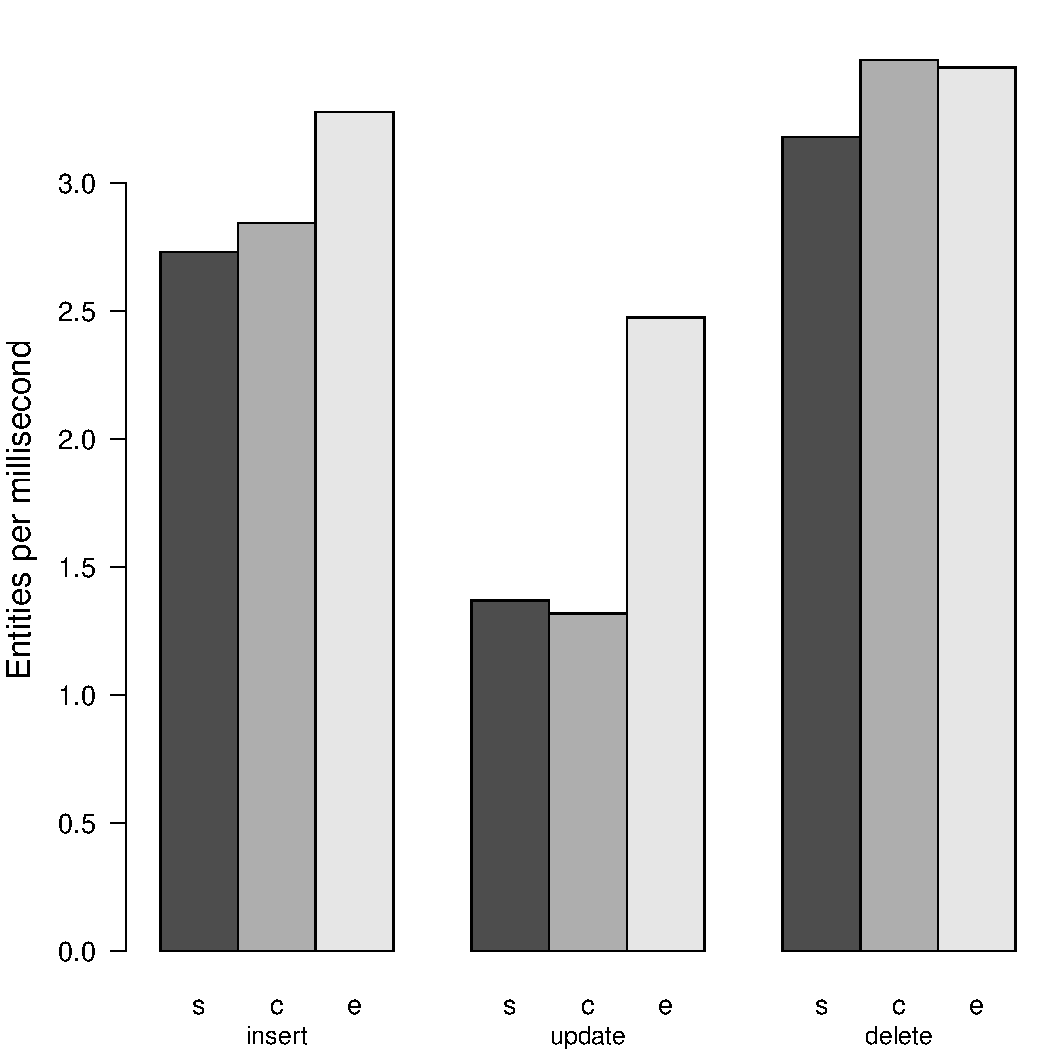
\includegraphics[width=\Width]{figure/result/barplot-Baseline-tp.pdf}\label{fres:Baseline-throughput}}
		\caption{Performance of Baseline}\label{fres:Baseline}
	\end{figure}
The performance of the  \texttt{insert} operation is expected to be similar
across solutions since no referential integrity validations are performed. However, the figure
shows a slightly  better average performance when inserting in
\texttt{Enrolment}. This subtle difference might be due to the smaller number of
columns as well as the smaller size of the contents that \texttt{Enrolment}
entities have when compared to \texttt{Course} and even more when compared to
\texttt{Student}. Also, external factors such as network latency are expected to
affect the performance slightly.

The performance of \texttt{delete} operations is similar across entities as
well, and quite similar to the performance of the \texttt{insert} operations.
This is because the tombstone delete paradigm in Cassandra does not allow a
complete removal of the super columns, but rather it keeps the row keys and
writes empty values to the columns to mark the super column as deleted. Thus, it
is expected as well to perform similar to the \texttt{insert} operations.


Finally, the performance of the \texttt{update} operation is worse
as it takes more time to complete because it involves  \texttt{insert} and
\texttt{delete} operations in the cases of \texttt{Course} and
\texttt{Student}. However, the \texttt{update} operation in \texttt{Enrolment}
is much better as it does not change the primary keys of these entities,
instead, since only the foreign keys are changed. Thus, this operation on
\texttt{Enrolment} acts as an \texttt{insert} operation.

%The performance of the operations when referential integrity validations are
%introduced  is compared with a baseline experiment where such operations  do not
%trigger any such validations.  This baseline serves as a reference to
%determine the difference in performance of the \ac{DBMS} when validations are
%imposed using the \ac{API} and to analyse the performance of the solutions.

% In the baseline experiment,  the operations on the entities represent how
% operations on data are performed in Cassandra without referential integrity
% validations. In order to be consistent with the solutions, the operations
% \texttt{Create}, \texttt{Update} and \texttt{Delete} for the baseline are
% measured in the same way operations are measured for the solutions and the
% artificial data for the baseline experiment is created the same way as well.
% Note that, \texttt{Create} inserts all the entities for \texttt{Student},
% \texttt{Course} and \texttt{Enrolment}.  \texttt{Update} performs changes on the
% primary keys of \texttt{Student} and \texttt{Course} entities,  and on the
% foreign keys (\texttt{CourseId}) of \texttt{Enrolment} while \texttt{Delete}
% removes all the \texttt{Student},  \texttt{Course} and \texttt{Enrolment}
% entities. These operations are performed precisely the same way as the
% solutions, so that the comparison and analysis of results are balanced and
% unbiased.
% 
% The results in terms of average response time and throughput for the baseline
% experiment are presented as  bar-plots in Figure~\ref{fres:Baseline}. 
% Specifically,  Figure~\ref{fres:Baseline-responsetime} shows the response time 
% of each operation on a single entity in the three column families and 
% Figure~\ref{fres:Baseline-throughput} presents the throughput of each operation
% on the same column families within one second. 
% % The analysis of the performance of each operation on an entity is discussed as
% % follows. 

% 	\begin{figure}[h] \centering
% 	\includegraphics[width=. 8\textwidth]{. /figure/result/barplot-Baseline-rt.pdf}
% 		\caption{Baseline}\label{fr:Solution0-barplot}
% 	\end{figure}
	


% As seen from these results,  the \texttt{delete} operation takes in average the
% lowest response time and the highest throughput.  That is,  the
% time to delete an entity is shorter when compared to \texttt{insert} or \texttt{update}, 
% which in turn means that more \texttt{delete} operations can be performed within
% a second.  On the other hand,  \texttt{update} takes the most time to complete all
% the operations thus providing a low throughput while \texttt{insert} is
% faster than \texttt{update} and quite similar to \texttt{delete}. 
% 
% % The \texttt{delete} operation performs faster than the other operations
% % because Cassandra performs  tombstone deletes,  where data is not physically
% % but only logically marked as deleted.
% The \texttt{update} operation takes the most time because it
% % because it requires searching by index to access the correct columns in the
% % column family.  Moreover,   an \texttt{update}
% involves  \texttt{insert} and
% \texttt{delete} operations in the cases of \texttt{Course} and \texttt{Student}
% hence taking more time that the other operations. However, the
% \texttt{update} in \texttt{Enrolment} takes similar time to other
% operations because it does not change the primary keys of these entities,
% instead, only the foreign keys are changed.  % On the other hand,
% % \texttt{update} on \texttt{Student} and \texttt{Course} entities changes the
% % primary keys,  which involves performing an \texttt{insert} and a
% % \texttt{delete} operation for each entity.
% % The \texttt{insert} operation takes slightly more time than \texttt{delete}
% % since data has to be physically written into the column families.
% 
% The time taken to insert and delete entities from \texttt{Student}, 
% \texttt{Course} and \texttt{Enrolment} are rather similar since there are no
% referential integrity validations.  However, the slight differences might be 
% due to differences in number of columns,  size of contents or even external
% factors.






